\chapter{Experiments} \label{chapt:Experiments}

In this chapter we experimentally validate the novel drift detectors we have introduced, and investigate the performance of drift detectors on a synthetic medical triage dataset. Section \ref{Experiments:details} specifies the details which of the experiments which will be run in this chapter. Section \ref{Experiments:bernoulli} describes some experiments with Bernoulli data streams which validate the approach taken by CDDM. Section \ref{Experiments:benchmark} investigates the performance of our drift detectors on a battery of benchmark data streams. Section \ref{Experiments:triage} introduces a data stream which simulates a medical referral triage environment, and investigates the performance of our drift detectors on this dataset. Section \ref{Experiments:conclusion} summarises this chapter and discusses future work.

%-------------------------------------------------------------------
% EXPERIMENT DETAILS
%-------------------------------------------------------------------

\section{Experiment Details} \label{Experiments:details}

This section provides details of the experiments which will be performed in the following sections. The experiments are implemented using a modified version of the Tornado framework \cite{tornado}. The experiments are performed on a 2.5 GHz Intel Core i7 with 16GB RAM. The operating system is macOS Mojave version 10.14.6. 

Within each experiment suite, we run all the drift detectors which are in Tornado. These are ADWIN \cite{ADWIN}, CUSUM \cite{CUSUM}, DDM \cite{DDM}, EDDM \cite{EDDM}, EWMA \cite{EWMA}, FHDDM \cite{FHDDM}, FHDDMS \cite{FHDDM}, FHDDMS$_{add}$ \cite{FHDDM}, HDDM$_A$ \cite{HDDM}, HDDM$_W$ \cite{HDDM}, MDDM$_A$ \cite{HDDM}, MDDM$_E$ \cite{MDDM}, MDDM$_G$ \cite{MDDM}, PH \cite{CUSUM}, RDDM \cite{RDDM}, and SeqDrift2 \cite{seq_drift}. CUSUM and PH are not the original procedure proposed by Page \cite{CUSUM}, but the modified versions described in \cite{gama_survey}. We compare these existing drift detectors with our novel detectors, BWAF and CDDM. We do not test BDDM due to it being $O(t^2)$ and therefore inappropriate for data streams.

This covers the most popular drift detection methods, although there are some notable omissions. All of these methods use the error-rate operationalisation of concept drift, so LFR \cite{LFR} which is a state-of-the-art detector with an alternative operationalisation would have been a sensible comparison to CDDM. Similarly, BCMC is a Bayesian approach to concept drift detection, so would have been useful to compare to BWAF. However, to our knowledge, code for these detection methods is not publicly available.

Unless otherwise stated, the experiments are run using the three most popular models implemented in Tornado. These are the perceptron \cite{perceptron}, the na\"{i}ve Bayes, and the Hoeffding tree \cite{hoeffding_trees}.

We evaluate the performance of detectors using the following metrics. A drift signal emitted by the drift detector within 250 time steps of a concept drift, is interpreted as a true positive (TP). A failure to emit a drift signal within 250 time steps of a concept drift is interpreted as a false negative (FN). A drift signal which is emitted when a concept drift has not occurred in the last 250 time steps is interpreted as a false positive (FP).  

The {\bf precision} of the detector is given by
\begin{equation}
    \text{Precision} = \frac{N_{TP}+1}{N_{TP}+N_{FP}+2}
\end{equation}
where $N_{TP}$ is the number of true positives, and similarly for $N_{FP}$ and $N_{FN}$. Note that this formula makes use of Laplace smoothing to avoid division-by-zero errors. The {\bf recall} of the detector is given by
\begin{equation}
    \text{Recall} = \frac{N_{TP}+1}{N_{TP}+1+N_{FN}+1}
\end{equation}
The {\bf F$_1$} score of the drift detector is given by
\begin{equation}
    F_1 = \frac{2}{\text{Precision}^{-1}+\text{Recall}^{-1}}.
\end{equation}
The {\bf mean delay} is the mean number of time steps between a concept drift occurring and a drift signal being emitted. Because any signals after 250 time steps are considered false positives, this is the maximum value for mean delay. {\bf Memory} is the memory footprint of the drift detector in bytes measured at the end of an experimental trial. {\bf Runtime} is the number of milliseconds between the beginning and end of the experimental trial.

Results are reported in tables in the form ``mean (std)", where ``std" is the sample standard deviation across the experimental trials. The best detector on each metric is rendered in bold. The results are additionally visualised using CD diagrams \cite{cd_diagrams}.

%-------------------------------------------------------------------
% BERNOULLI
%-------------------------------------------------------------------

\section{Bernoulli Experiments} \label{Experiments:bernoulli}

In this section we describe experiments on a data stream which validates the benefit of CDDM's approach to concept drift detection. Specifically, we show how the pathologies discussed in Section \ref{CDDM:motivation} of false positive and false negative drift detections can occur from feature drift and variation in the difficulty of in prediction tasks.

% \subsection{Setting}

In this data stream, instances consist of a single Bernoulli feature $x$. Labels $y$ are likewise Bernoulli variables, whose rate depends on the feature value:
\begin{align}
  \Pr(x=i) &= \begin{cases}
    1-\gamma & \text{if }x=0 \\
    \gamma & \text{if }x=1.
    \end{cases} \\
  \Pr(y=1|x=i) &= \begin{cases}
    \alpha & \text{if }x=0 \\
    \beta & \text{if }x=1.
    \end{cases}
\end{align}
We will call $\gamma$ the feature rate, and $\alpha$ and $\beta$ the label rates. The instance-label joint probability of the data stream is illustrated in Figure \ref{fig:bernoulli}.

We are interested in two kinds of concept drift. First we have feature drift, in which the feature rate changes, but the label rates remain the same.
\begin{equation}
  (\gamma,\alpha,\beta) \Rightarrow (\gamma',\alpha,\beta)
\end{equation}
Second, we have real drift concurrent with virtual drift, in which the feature rate, {\it and} the label rates change. 
\begin{equation}
  (\gamma,\alpha,\beta) \Rightarrow (\gamma',\alpha',\beta')
\end{equation}
When a drift detector is triggered by real drift, this is a true positive. When a drift detector is triggered by feature drift, this is a false positive. Our experiments with Bernoulli data streams consist of 1000 time steps under the pre-drift distribution, followed 1000 time steps in the post-drift distribution. %If a drift detector is triggered after a real drift, then a count of true positives is incremented. If a detector is triggered before a real drift, or after a virtual drift, then a count of false positives is incremented. If a detector is not triggered after a real drift before the 1250 time steps have completed, then a count of false negatives is incremented. 
%We run 400 iterations of each data stream. 

We use na\"{i}ve Bayes as our learner. Na\"{i}ve Bayes' are known to be poorly calibrated \cite{calibrating}, so are typically a poor choice to use with CDDM. However, given this data stream has one-dimensional instances, the usual issues of independence assumptions between features does not arise. % Na\"{i}ve Bayes is an acceptable model to use with CDDM on this data stream.

In this data stream, we have one feature value whose label is hard to predict, and one feature value whose label is easy to predict. Specifically, a feature an $x=0$ instance is consistently labelled as $y=0$, with no noise. A feature value of $x=1$ is also labelled as $y=0$, but with a noise rate 0.2. The feature rate is uniformly sampled for each instance of the data stream.
\begin{align}
  \alpha &= 0 \\
  \beta &= 0.2 \\
  \gamma &\sim U[0,1]
\end{align}
Virtual drift is implemented by reversing the feature rate. 
\begin{equation}
  (\gamma,\alpha,\beta) \Rightarrow (1-\gamma,\alpha,\beta)
\end{equation}
Real drift is implemented by reversing the feature rate {\it and} reversing the first label rate.
\begin{equation}
  (\gamma,\alpha,\beta) \Rightarrow (1-\gamma,1-\alpha,\beta)
\end{equation}
These two scenarios are illustrated in Figure \ref{fig:bernoulli_hard}.

\begin{figure}
    \centering
    % \includegraphics[width=0.5\textwidth]{images/bernoulli.jpg}
    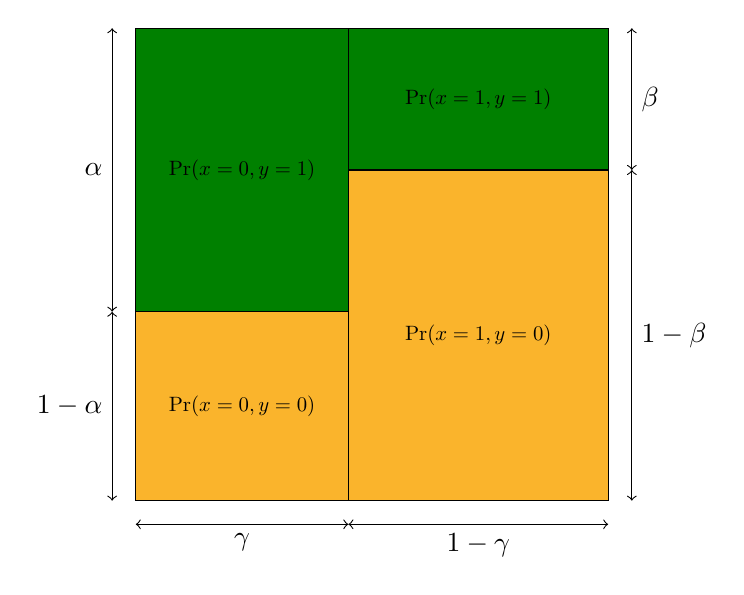
\begin{tikzpicture}[scale=6]
        %--- Arguments ----
        \def \g {0.45} % gamma
        \def \a {0.6} % alpha
        \def \b {0.3} % beta
        \def \zeroColor {Dandelion} % colour of y=0 boxes
        \def \oneColor {Green} % colour of y=1 boxes
        \def \textsep {0.05}
        %--- Rectangles ---
        \draw [fill=\zeroColor] (0,0) rectangle (\g,1-\a);
        \draw [fill=\oneColor] (0,1-\a) rectangle (\g,1);
        \draw [fill=\zeroColor] (\g,0) rectangle (1,1-\b);
        \draw [fill=\oneColor] (\g,1-\b) rectangle (1,1);
        %--- Lines ---
        % alpha
        \draw [<->] (-\textsep, 0) -- (-\textsep, 1-\a);
        \draw [<->] (-\textsep, 1-\a) -- (-\textsep, 1);
        % gamma
        \draw [<->] (0, -\textsep) -- (\g, -\textsep);
        \draw [<->] (\g, -\textsep) -- (1,-\textsep);
        % beta
        \draw [<->] (1+\textsep, 0) -- (1+\textsep, 1-\b);
        \draw [<->] (1+\textsep, 1-\b) -- (1+\textsep, 1);
        %--- Outer labels ---
        % alpha
        \node [left] at (-\textsep, 0.5-\a/2) {$1-\alpha$};
        \node [left] at (-\textsep, 1-\a/2) {$\alpha$};
        % gamma
        \node [below] at (\g/2,-\textsep) {$\gamma$};
        \node [below] at (0.5+\g/2,-\textsep) {$1-\gamma$};
        % beta
        \node [right] at (1+\textsep, 0.5-\b/2) {$1-\beta$};
        \node [right] at (1+\textsep, 1-\b/2) {$\beta$};
        %--- Inner labels ----
        \node [scale=0.75] at (\g/2,0.5-\a/2) {$\Pr(x=0,y=0)$};
        \node [scale=0.75] at (\g/2,1-\a/2) {$\Pr(x=0,y=1)$};
        \node [scale=0.75] at (0.5+\g/2,0.5-\b/2) {$\Pr(x=1,y=0)$};
        \node [scale=0.75] at (0.5+\g/2,1-\b/2) {$\Pr(x=1,y=1)$};
    \end{tikzpicture}
    \caption{Distribution of the Bernoulli data stream.}
    \label{fig:bernoulli}
\end{figure}

\begin{figure}
    \centering
    % \includegraphics[width=0.5\textwidth]{images/bernoulli_hard.jpg}
    \begin{tikzpicture}[scale=4]
        % --- DEFINITIONS ---
        \def \xSep {2}
        \def \ySep {1.5}
        \def \arrowSep {0.2}
        \def \textSep {0.2}
        \def \gZero {0.25}
        \def \gOne {0.75}
        \def \bZero {0.7}
        \def \bOne {0.3}
        \def \zeroColor {Dandelion} % colour of y=0 boxes
        \def \oneColor {Green} % colour of y=1 boxes
        % \def \zeroColor {Dandelion} % colour of y=0 boxes
        % \def \oneColor {Green} % colour of y=1 boxes
        \newcommand{\bernSqr}[4]{
            % draw a Bernoulli square
            % args:
            %  x value of bottom left
            %  y value of bottom left
            %  gamma
            %  beta
            \draw [fill=\oneColor] (#1,#2) rectangle (#1+#3,#2+1);
            \draw [fill=\zeroColor] (#1+#3,#2) rectangle (#1+1,#2+1-#4);
            \draw [fill=\oneColor] (#1+#3,#2+1-#4) rectangle (#1+1,#2+1);
        }
        % --- SQUARES ---
        \bernSqr{0}{0}{\gZero}{\bZero}
        \bernSqr{\xSep}{0}{\gOne}{\bOne}
        \bernSqr{0}{\ySep}{\gZero}{\bZero}
        \bernSqr{\xSep}{\ySep}{\gOne}{\bZero}
        % --- ARROWS ---
        \draw [ultra thick, ->] (1+\arrowSep,0.5) -- (\xSep-\arrowSep,0.5);
        \draw [ultra thick, ->] (1+\arrowSep,\ySep+0.5) -- (\xSep-\arrowSep,\ySep+0.5);
        % --- TEXT ---
        \node at (0.5+\xSep/2,-\textSep) {Real drift};
        \node at (0.5+\xSep/2,\ySep-\textSep) {Feature drift};
    \end{tikzpicture}
    \caption{Distributional changes in the Bernoulli data stream.}
    \label{fig:bernoulli_hard}
\end{figure}

If the initial feature rate is less than 0.5, then after virtual drift we will see an increase in the error rate of the model due to an increase in the rate of ``hard problems". 

Conversely, when the feature rate is greater than 0.5, when real drift occurs we will see a decrease in the rate of ``hard problems", which will decrease the error rate. This may hide the increase in the error rate due to the real drift itself, and can lead to false negatives. 

More specifically, the change in error rate due to feature drift will be positive when
\begin{align}
  0 &< \Delta E \\
  &< (1-\gamma)\beta - \gamma \beta \\
  &< \beta-2\gamma\beta \\
  \gamma &< 0.5.
\end{align}
Thus, any feature rate greater than 0.5 may trigger false positives in error-rate detectors. The change in error rate due to real drift is positive when
\begin{align}
  0 &< \Delta E \\
  &< (1-\gamma)(1-\beta) - \gamma\beta \\
  &< 1 - \gamma - \beta \\
  \gamma &< 0.8.
\end{align}
Thus false negatives may occur when the feature rate is above 0.8.

The results of the trials on this data stream are given in Table \ref{tab:bernoulli}, and illustrated in Figure \ref{fig:bernoulli_cd}. CDDM achieves the highest precision and F$_1$ score of any of the detectors (although not significantly greater than the runner up at $p<0.05$ significance). 

\begin{sidewaystable}
    \centering
    \caption{Results of Bernoulli datasets.}
    \input{tables/bernoulli.tex}
    \label{tab:bernoulli}
\end{sidewaystable}

\begin{figure}
    \centering
    \includegraphics[width=\textwidth]{images/cd_diagrams/bernoulli.pdf}
    \caption{CD diagram of Bernoulli datasets.}
    \label{fig:bernoulli_cd}
\end{figure}

%-------------------------------------------------------------------
% BENCHMARK DATASETS
%-------------------------------------------------------------------

\section{Benchmark Datasets} \label{Experiments:benchmark}

In this section we evaluate the concept drift detection methods we have introduced on a battery of benchmark datasets. The Tornado framework provides implementations of the following synthetic data streams:
\begin{itemize}
    \item {\bf CIRCLES} Each instance consists of two attributes $x_1,x_2\sim U[0,1]$. Each concept consists of three values, $r,x_{circ},y_{circ}\in[0,1]$, representing the radius of a circle, and $x$ and $y$ coordinates of the center of a circle. And instance is given a positive label if it falls within the circle, otherwise it is given a negative label. Sampling is done such that an equal number of positive and negative instances occur. The concept parameters cycle through the values of $[0.15, 0.2, 0.5]$, $[0.2, 0.4, 0.5]$, $[0.25, 0.6, 0.5]$ and $[0.3, 0.8, 0.5]$.
    \item {\bf LED} Each concept in the LED task is a digit displayed on a 7-bit LED interface. There are 10 labels (the digits $0,1,2,\dots,9$) and 7 binary features (each of the display bits).  For example, the label corresponding to the instance [1, 1, 1, 1, 1, 1, 0] is $0$. In addition to the concept bits, there are also $n$ irrelevant and random-valued binary attributes. The position of the irrelevant attributes changes with each concept, so the model must learn anew which attributes are decision-relevant. 
    \item {\bf MIXED} Each instance is a mix of two binary attributes $w,v\in\{0,1\}$, and two real-valued attributes $x_1,x_2\sim U[0,1]$. Labels are assigned according to $y=\mathrm{1}[v \wedge w \wedge  y < 0.5 + 0.3 \sin(3\pi x)]$. After each context change the classification is reversed.
    \item {\bf SEA} Each instance consists of three attributes $x_1,x_2,x_3\sim U[0,10]$. Each concept consists of a threshold $\theta$, such that $y=\mathrm{1}[x_1+x_2+x_3 > \theta]$. That is, if the binary label denotes whether the sum of the attributes exceeds the threshold. Thresholds cycle between the values $[8, 9, 7, 9.5]$.
    \item {\bf SINE1} Each instance consists of two attributes $x_1,x_2\sim U[0,1]$. Binary labels are given by $y = \mathrm{1}[x_1>sin(x_2)]$. When concept drift occurs, the labels are reversed.
    \item {\bf SINE2} As with SINE1, the attributes are $x_1,x_2\sim U[0,1]$. Binary labels are given by $y = \mathrm{1}[x_1>0.5+0.3\sin(3\pi x_2)]$. When concept drift occurs, the labels are reversed.
    \item {\bf STAGGER} Instances consist of categorical attributes $size\in [small, medium, large]$, $color\in [red, green]$, $shape\in [circular, non-circular]$. Each concepts is a first order logic expression. Specifically, the following concepts are cycled: $y=\mathrm{1}[size=small \wedge color=red]$, $y=\mathrm{1}[color=green \vee shape=circular]$, and $y=\mathrm{1}[size=medium \vee size=large]$.
\end{itemize}
These data streams provide constitute the most popular benchmarks used in the concept drift detection literature. Each of these data streams has the following parameters:
\begin{itemize}
    \item {\bf Concept Length} The number of instances between concept drifts. If this number is small then the data stream is {\it volatile}, if this number is small then the data stream is {\it stable}.
    \item {\bf Transition Length} The number of instances over which a concept drift occurs. If the transition length is $n$, and there have been $i$ instances since the concept drift, then the probability that the new concept is used is $\Pr(new-concept)=i/n$, otherwise the previous concept is used. If the transition length is low then the drift is {\it abrupt}. Otherwise the stream is {\it gradual}.
    \item {\bf Noise Rate} The rate at which any given label will be replaced with a different label. For binary labels, the label is simply inverted. Otherwise, a different label is chosen at random. If this quantity is high, then the data stream is {\it noisy}.
\end{itemize}
We are interested in how drift detector performance varies with noise and transition length. We therefore run experiments using each of the variations of the above datasets
\begin{itemize}
    \item {\bf High Noise} Noise rate is set to 0.4, transition length is set to 50 and concept length is set to 1000.
    \item {\bf Low Noise} Noise rate is set to 0.02, transition length is set to 50 and concept length is set to 1000.
    \item {\bf Gradual Drift} Transition length is set to 250, noise rate is set to 0.1, and concept length is set to 1000.
    \item {\bf Abrupt Drift} Transition length is set to 0, noise rate is set to 0.1, and concept length is set to 1000.
    \item {\bf Long concepts} Transition length is set to 50, noise rate is set to 0.1, and concept length is set to 25000.
    \item {\bf Short concepts} Transition length is set to 50, noise rate is set to 0.1, and concept length is set to 250.
\end{itemize}
We run each datastream with two base learners. Na\"{i}ve Bayes and Hoeffding trees \cite{hoeffding_trees} are two of the most popular, so we use these.  

We run two iterations of each of the 7 data streams, for each of the four variations, with both of the base learners. The results are given in Table \ref{tab:benchmarks} and visualised in Figure \ref{fig:benchmarks}. 

\begin{sidewaystable}
    \centering
    \caption{Results of benchmark datasets.}
    \input{tables/benchmark.tex}
    \label{tab:benchmarks}
\end{sidewaystable}

\begin{figure}
    \centering
    \includegraphics[width=\textwidth]{images/cd_diagrams/benchmark.pdf}
    \caption{CD diagram of benchmark datasets.}
    \label{fig:benchmarks}
\end{figure}

We see that BWAF performs well on benchmark datasets. It achieves the fifth highest precision (significantly less than the best detector at $p<0.05$), the seventh best recall (not significantly less than the best detector at $p<0.05$), the fourth best F$_1$ score (not significantly less than the best detector at $p<0.05$), the best mean delay (although not significantly greater than the second best at $p<0.05$), the fifth best memory consumption (not significantly worse than the best detector at $p<0.05$), but the second worst runtime.

By contrast, the performance of CDDM is poor. Because the instances in these data streams are high dimensional, the learners are uncalibrated, triggering a high rate of false positives. On recall and memory, CDDM is ranked in the middle the detectors. On all other metrics it is in the lower half of detectors. This affirms the statement in Section \ref{CDDM:conclusion} that CDDM must be extended with online calibration for practical usage.

%-------------------------------------------------------------------
% SYNTHETIC MEDICAL
%-------------------------------------------------------------------

\section{Triage Simulation} \label{Experiments:triage}

In this section we evaluate our novel concept drift detectors in the motivating example domain of GP referrals triage. Due to a lack of real triage data annotated by concept drift, we instead use a synthetic data stream with concept drift deliberately introduced.

We base our synthetic data stream on the MIMIC-III dataset - a publicly available repository of free-text electronic health records \cite{mimic}. There are several types of documents within the dataset, so we limit our usage to `radiology' documents, which have the advantage of having structured headers. We preprocess the 522,279 radiology documents by converting the text into bag-of-words format. To keep the instance dimensionality reasonable, we eliminate tokens which occur in fewer than 40\% or more than 60\% of documents, resulting in 59,652 dimensional features. We shuffle the order of the documents to make sure the only concept drifts which occurs in the data stream have been deliberately engineered.

To simulate a triage rule, we randomly label 30 referral documents with priority labels 1 to 4. We then train a decision tree on these instance-label pairs. We repeat this several times to obtain a set of ``triage concepts". Concept drift is simulated by labelling the instances prior to the drift point using one triage concept, and then labelling the instances after the drift with another, randomly selected concept. In each instantiation of the data stream a single concept drift occurs halfway through the stream.

We run two iterations of the medical triage data stream under each of the variations described in Section \ref{Experiments:benchmark}, namely high noise, low noise, gradual drift, abrupt drift, long concepts, short concepts. The results are given in Table \ref{tab:triage} and visualised in Figure \ref{fig:triage}. 

\begin{sidewaystable}
    \centering
    \caption{Results of synthetic triage data streams.}
    \input{tables/mimic.tex}
    \label{tab:triage}
\end{sidewaystable}

\begin{figure}
    \centering
    \includegraphics[width=\textwidth]{images/cd_diagrams/mimic.pdf}
    \caption{CD diagram of synthetic triage data streams.}
    \label{fig:triage}
\end{figure}

Similar to Section \ref{Experiments:benchmark}, we see competitive performance from BWAF. It achieves the second highest precision, recall, and F$_1$ score, as well as the third best mean delay (none of which is significantly worse than the best detector at $p<0.05$). The memory consumption is sixth best (not significantly less than the best detector at $p<0.05$), although the runtime is fifth worst.

As in Section \ref{Experiments:benchmark}, the performance of CDDM is poor. CDDM achieved the worst precision and F$_1$ of all the detectors, although it achieved the sixth best recall, the best mean delay, the second best memory consumption, and the third lowest runtime. As before, this poor performance can be attributed to the models being miscalibrated, a problem which is especially acute given the high dimensionality of the data. 

%-------------------------------------------------------------------
% CONCLUSION
%-------------------------------------------------------------------

\section{Conclusion} \label{Experiments:conclusion}

In this chapter we experimentally validated our novel drift detectors, and investigated the performance of drift detectors on a synthetic medical triage dataset. We have seen that CDDM can achieve leading precision F$_1$ and precision scores on Bernoulli streams with feature drift and uneven noise. We have also seen that BWAF is a competitive drift detector on a battery of benchmark data streams, and a synthetic GP referrals triage data stream. It consistently achieved one of the best precision, recall, F$_1$, detection delays scores. BWAF's memory usage reasonable, consistently within the top quartile, although its runtime was generally not competitive. CDDM did not perform competitively in these experiments. We attribute this to the models being uncalibrated, thus affirming the claim made in Section \ref{CDDM:conclusion} that CDDM should be combined with online calibration for practical usage.